%! Author = zhenxiang
%! Date = 23-3-30

\PassOptionsToPackage{quiet}{xeCJK}  % 抑制无意义的警告
% Preamble
\documentclass[11pt]{ctexart}


% Packages
\usepackage{amsmath}
% graphicx
\usepackage{graphicx}
% 页面设置
\usepackage{geometry}
\geometry{left=2.5cm, right=2.5cm, top=2.5cm, bottom=2.5cm}
% codes
\usepackage{ listings}
\usepackage{xcolor}
\usepackage{color}
\definecolor{mygreen}{rgb}{0,0.6,0}
\definecolor{mygray}{rgb}{0.5,0.5,0.5}
\definecolor{mymauve}{rgb}{0.58,0,0.82}
\lstset{ %
	backgroundcolor=\color{white},   % choose the background color; you must add \usepackage{color} or \usepackage{xcolor}
	basicstyle=\ttfamily,            % the size of the fonts that are used for the code
	breakatwhitespace=false,         % sets if automatic breaks should only happen at whitespace
	breaklines=true,                 % sets automatic line breaking
	captionpos=b,                    % sets the caption-position to bottom
	commentstyle=\ttfamily\color{mygreen},    
	% comment style
	deletekeywords={},               % if you want to delete keywords from the given language
	escapeinside={},                 % if you want to add LaTeX within your code
	extendedchars=true,              % lets you use non-ASCII characters; for 8-bits encodings only, does not work with UTF-8
	frame=single,                    % adds a frame around the code
	keepspaces=true,                 % keeps spaces in text, useful for keeping indentation of code (possibly needs columns=flexible)
	keywordstyle=\color{blue},       % keyword style
	language=C++,                    % the language of the code
	morekeywords={},                 % if you want to add more keywords to the set
	numbers=left,                    % where to put the line-numbers; possible values are (none, left, right)
	numbersep=5pt,                   % how far the line-numbers are from the code
	numberstyle=\tiny\color{mygray}, % the style that is used for the line-numbers
	rulecolor=\color{black},         % if not set, the frame-color may be changed on line-breaks within not-black text (e.g. comments (green here))
	showspaces=false,                % show spaces everywhere adding particular underscores; it overrides 'showstringspaces'
	showstringspaces=false,          % underline spaces within strings only
	showtabs=false,                  % show tabs within strings adding particular underscores
	stepnumber=1,                    % the step between two line-numbers. If it's 1, each line will be numbered
	stringstyle=\color{mymauve},     % string literal style
	tabsize=2,                       % sets default tabsize to 2 spaces
	title=\lstname                   % show the filename of files included with \lstinputlisting; also try caption instead of title
}

% Document
\begin{document}

\section{Reading}

\subsection{Memory and data locality}

迄今为止,我们已经学习了如何编写CUDA内核函数以及如何通过大量线程配置和协调其执行。在本章中,我们将研究如何组织和定位数据,以便大量线程可以高效地访问它们。在第二章《数据并行计算》中,我们讨论了数据首先从主机内存传输到设备全局内存。在第三章《可伸缩并行执行》中,我们确定了如何使用块索引和线程索引使线程从全局内存中访问其数据部分。我们还探索了资源分配和线程调度。虽然我们所涵盖的范围是一个很好的起点,但我们迄今学到的CUDA内核函数可能只能实现底层硬件潜在速度的一小部分。这种性能低下归因于全局内存的长延迟(数百个时钟周期)和有限访问带宽,通常使用动态随机访问存储器实现。虽然有大量的线程可用于执行,理论上可以容忍长时间的内存访问延迟,但您很容易会遇到一种情况,即全局内存访问路径中的交通拥塞阻止了除少数线程以外的所有线程取得进展,从而使一些流多处理器(SMs)闲置。为了避免这种拥塞,CUDA提供了许多额外的资源和访问内存的方法,可以消除大部分与全局内存的交通。在本章中,您将学习使用不同类型的内存来提高CUDA内核函数的执行效率。

\subsubsection{IMPORTANCE OF MEMORY ACCESS EFFICIENCY}

在下面这串代码,其中\ verb|pixVal += in[curRow * w + curCol]| 这行代码,全局内存访问获取一个in[]数组元素,浮点加法操作是pixVal+=

因此浮点计算与全局内存访问操作的比率是1:1,即1.0,我们将这个比率称为计算-全局内存访问比率,它表示在程序的某个区域内执行每次访问全局内存所需执行的浮点计算数量。

计算-全局内存访问比率对CUDA内核的性能有重要影响。
In a high-end(高端) device today, the global memory bandwidth is around 1,000 GB/s, or 1 TB/s. With four bytes in each single-precision
floating-point value, no more than 1000/4 = 250 giga single-precision operands per
second can be expected to load. With a compute-to-global-memory ratio of 1.0, the
execution of the image blur kernel will be limited by the rate at which the operands
(e.g., the elements of in[]) can be delivered to the GPU. We will refer to programs
whose execution speed is limited by memory access throughput as memory-bound
programs. In our example, the kernel will achieve no more than 250 giga floating-
point operations per second (GFLOPS).

在当今高端设备中,全局内存带宽约为1,000 GB/s或1 TB/s。每个单精度浮点值占用4个字节,因此最多可以期望加载1000/4=250 giga单精度操作数每秒。如果计算-全局内存比率为1.0,则图像模糊内核的执行将受到将操作数(如in[]的元素)传输到GPU的速率的限制。我们将执行速度受内存访问吞吐量限制的程序称为内存限制程序。在我们的示例中,内核的执行速度将不会超过250 giga浮点操作每秒(GFLOPS)。
虽然250 GFLOPS是一个可观的数字,但它仅是高端设备峰值单精度性能12 TFLOPS或更高的微不足道的一部分(2\%)。为了实现更高水平的内核性能,我们需要通过减少全局内存访问的数量来增加计算-全局内存比率。要实现处理器的峰值12 TFLOPS评级,我们需要48或更高的比率。一般来说,随着计算吞吐量增长速度快于内存带宽,过去几代设备中所需的比率已经在增加。本章的其余部分介绍一种常用的减少全局内存访问次数的技术。




\begin{lstlisting}
	__global__
void blurKernel(unsigned char * in, unsigned char * out, int w, int h){
	int Col  = blockIdx.x * blockDim.x + threadIdx.x;
	int Row = blockIdx.y * blockDim.y + threadIdx.y;
	
	if (Col < w && Row < h) {
		int pixVal = 0;
		int pixels = 0;	
		// Get the average of the surrounding BLUR_SIZE x BLUR_SIZE box
		for (int blurRow = - BLUR_SIZE; blurRow < BLUR_SIZE + 1; ++blurRow) {
			int curRow = Row + blurRow;
			int curCol = Col + blurCol;
			// Verify we have a valid image pixel
			if(curRow > -1 && curRow < h && curCol > -1 && curCol < w) {
				pixVal += in[curRow * w + curCol];
				pixels++; // Keep track of number of pixels in the avg	
			}		
			
		}
	}
	// Write our new pixel value out
	out[Row * w + Col] = (unsigned char)(pixVal /pixels); 
	
}

}



\end{lstlisting}

\subsubsection{MATRIX MULTIPLICATION}



矩阵乘法,在每次迭代中,需要执行两次全局内存访问以进行一次浮点数乘法和一次浮点数加法。一次全局内存访问获取一个M元素,另一次获取一个N元素。一次浮点数操作乘以获取的M和N元素,另一次将乘积累加到Pvalue中。因此,循环的计算与全局内存访问比率为1.0。

\begin{lstlisting}
	__global__ void MatrixMulKernel(float* M, float* N, float* P,
	int Width) {
		// Calculate the row index of the P element and M
		int Row = blockIdx.y*blockDim.y+threadIdx.y;
		// Calculate the column index of P and N
		int Col = blockIdx.x*blockDim.x+threadIdx.x;
		if ((Row < Width) && (Col < Width)) {
			float Pvalue = 0;
			// each thread computes one element of the block sub-matrix
			for (int k = 0; k < Width; ++k) {
				Pvalue += M[Row*Width+k]*N[k*Width+Col];
			}
			P[Row*Width+Col] = Pvalue;
		}
	}
\end{lstlisting}


\subsubsection{CUDA MEMORY TYPES}

在CUDA设备中,有几种类型的内存可以帮助程序员提高计算与全局内存访问比率,从而实现高执行速度。

% 图片置于当前位置
\begin{figure}[ht]
	\centering
	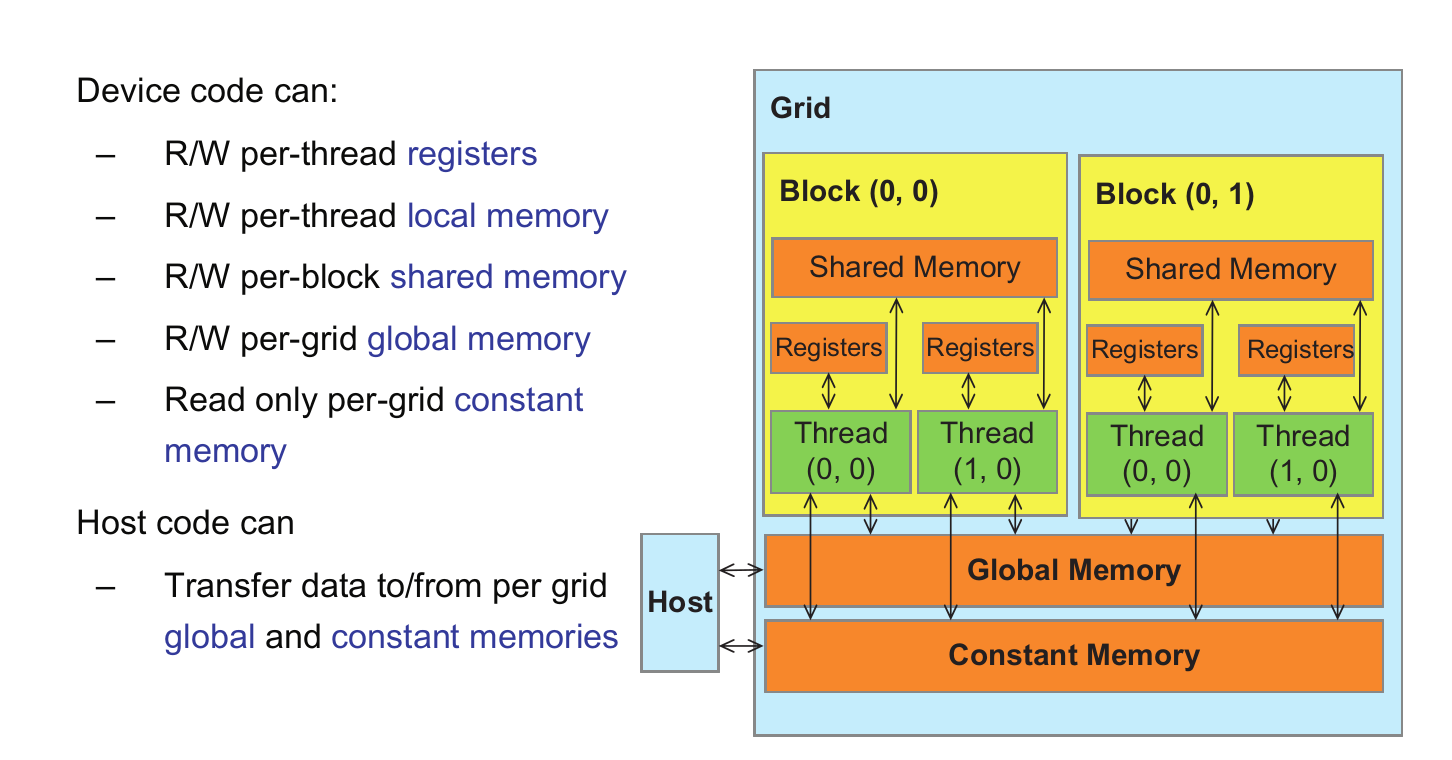
\includegraphics[width=1.0\textwidth]{images/OverviewoftheCUDAdevicememorymodel.png}
	\caption{Overview of the CUDA device memory model}
	\label{fig:1}
\end{figure}


\begin{itemize}
	\item  Global memory
	\item  Constant memory
	\item  Registers and shared memory
\end{itemize}

常量内存支持设备进行短延迟、高带宽的只读访问,寄存器和共享内存在芯片上。

驻留在这些类型的内存中的变量可以以非常高的速度以高度并行的方式进行访问。寄存器分配给各个线程;每个线程只能访问自己的寄存器。内核函数通常使用寄存器来保存每个线程私有的频繁访问的变量。共享内存位置分配给线程块;块中的所有线程都可以访问分配给块的共享内存变量。共享内存是线程通过共享其输入数据和中间结果相互合作的有效手段。通过在CUDA内存类型中声明CUDA变量,CUDA程序员可以指定变量的可见性和访问速度。

Q:线程块的size不是自己定义的吗?也就说共享内存的大小是灵活的吗

A: 是的,线程块的大小是由程序员自己定义的,可以在启动 CUDA kernel 函数时指定。因此,共享内存的大小也是可以灵活设定的,程序员可以根据需要定义合适的大小。共享内存的大小和线程块的大小有一定关系,因为共享内存是分配给线程块的,所以线程块的大小会影响共享内存的大小。一般来说,线程块的大小越大,分配给它的共享内存也就越大。但是需要注意的是,共享内存的大小也受到硬件限制,因此程序员需要根据硬件的实际情况来设定线程块和共享内存的大小,以达到最佳的性能。

为了完全理解寄存器、共享内存和全局内存之间的区别,我们需要更详细地了解这些不同类型的内存在现代处理器中是如何实现和使用的。几乎所有现代处理器都源于1945年由约翰·冯·诺伊曼提出的模型,该模型显示在图4.7中。CUDA设备也不例外。CUDA设备中的全局内存映射到图4.7中的Memory框。处理器框对应于我们今天通常看到的处理器芯片边界。全局内存位于处理器芯片外部,并采用DRAM技术实现,这意味着访问延迟长,访问带宽相对较低。寄存器对应于冯·诺伊曼模型的寄存器文件。寄存器文件位于处理器芯片上,这意味着访问延迟非常短,访问带宽比全局内存高得多。在典型设备中,寄存器文件的聚合访问带宽至少比全局内存高两个数量级。此外,当变量存储在寄存器中时,它的访问不再消耗芯片外的全局内存带宽。这种减少的带宽消耗将反映为增加的计算对全局内存访问比。

一个更微妙的问题是,每次访问寄存器需要的指令数比访问全局内存少。大多数现代处理器的算术指令都有“内置”的寄存器操作数。例如,浮点加法指令可能采用以下形式:

fadd r1,r2,r3

其中r2和r3是寄存器号,指定寄存器文件中存储输入操作数值的位置。存储浮点加法结果值的位置由r1指定。因此,当算术指令的操作数在寄存器中时,不需要额外的指令来将操作数值提供给算术逻辑单元(ALU),其中执行算术计算。

Q: CPU GPU的寄存器又有什么区别与联系

A: GPU和CPU的寄存器在作用和功能上是相似的,它们都是用来存储指令和数据的临时存储器。然而,由于GPU和CPU的体系结构和用途不同,它们的寄存器在一些方面存在区别。

首先,GPU上的寄存器数目通常比CPU多得多。这是因为GPU是设计用来处理大规模数据并行的任务,每个线程都需要有自己的寄存器,以存储临时数据和中间结果。此外,GPU通常会有多个线程块同时执行,每个线程块都需要有自己的寄存器。

其次,GPU上的寄存器具有更快的访问速度和更低的访问延迟。这是因为GPU的寄存器通常是嵌入到芯片中的,与处理器核心的距离更近,访问速度更快。此外,GPU上的寄存器还通常会采用更快的存储技术,例如SRAM,以提高访问速度和响应时间。

最后,GPU上的寄存器通常是由编译器和程序员管理的,而不是由操作系统管理。这是因为GPU通常被用来执行高性能计算任务,需要更多的控制和优化来充分利用硬件资源。因此,程序员需要手动管理寄存器的使用和分配,以确保最大的性能和效率。

\subsubsection{A TILED MATRIX MULTIPLICATION KERNEL}

请注意,共享内存变量的范围是块。因此,为每个块创建一对Mds和Nds,并且块中的所有线程都可以访问相同的Mds和Nds非常重要,因为块中的所有线程都必须可以访问由它们的同行加载到Mds和Nds中的M和N元素,以便它们可以使用这些值来满足它们的输入需求。


\begin{lstlisting}
	__global__ void MatrixMulKernel(float* d_M, float* d_N, float* d_P,
	int Width) {
		
		__shared__ float Mds[TILE_WIDTH][TILE_WIDTH];
		__shared__ float Nds[TILE_WIDTH][TILE_WIDTH];
		
		int bx = blockIdx.x; int by = blockIdx.y;
		int tx = threadIdx.x; int ty = threadIdx.y;
		
		 // Identify the row and column of the d_P element to work on
		int Row = by * TILE_WIDTH + ty;
		int Col = bx * TILE_WIDTH + tx;
		
		float Pvalue = 0;
		// Loop over the d_M and d_N tiles required to compute d_P element
		for (int ph = 0; ph < Width/TILE_WIDTH; ++ph) {

		// Collaborative loading of d_M and d_N tiles into shared memory
		Mds[ty][tx] = d_M[Row*Width + ph*TILE_WIDTH + tx];
		Nds[ty][tx] = d_N[(ph*TILE_WIDTH + ty)*Width + Col];
		__syncthreads();

		for (int k = 0; k < TILE_WIDTH; ++k) {
				Pvalue += Mds[ty][k] * Nds[k][tx];
		}
		__syncthreads();

		}
		d_P[Row*Width + Col] = Pvalue;

	}
\end{lstlisting}

tiled算法提供了重大的优势。对于矩阵乘法而言,全局内存访问的量将减少 TILE\_WIDTH 倍。如果使用 16 x 16 的瓦片,则全局内存访问量可以减少 16 倍。这将将计算与全局内存访问的比率从 1 提高到 16。这种改进使得 CUDA 设备的内存带宽可以支持接近其峰值性能的计算速率。例如,具有 150 GB/s 全局内存带宽的设备可以达到 ((150/4)*16) = 600 GFLOPS!

尽管tiled矩阵乘法内核的性能提升非常卓越,但它包含了一些简化的假设。首先,假设矩阵的宽度是线程块宽度的倍数。这个假设会防止内核正确处理任意大小的矩阵。第二个假设是矩阵是方阵,这在现实生活中并不总是正确的。在下一节中,我们将介绍一个带有边界检查的内核,可以消除这些假设。

\subsubsection{BOUNDARY CHECKS}



\end{document}